\chapter{State of the art}
\textit{This chapter refers to (and summarizes) my Master project. Concepts and definitions are essentially inspired by the chapter 10 of the book ``Principles of model checking'' \cite{PMC}, the chapter ``Model checking probabilistic systems'' of the Mickael Randour course named ``Formal verification of computer systems'' \cite{MRV} as well as the article ``Variations on the stochastic shortest path problem'' \cite{DBLP:journals/corr/RandourRS14a}.} \\

Before studying different multi-objective problems in \textit{Markov decision
processes} and defining \textit{strategies} that solve such problems, we will introduce some fundamental concepts that define the area of the subject.
Actually, we will be interested to know some measurements related to the cost of \textit{paths} of Markov decision processes as well as to the probability to reach some states in these models through these paths.
These measurements can not be computed without defining a probability measure on events formed by these paths.
So, first of all, we need to define what are \textit{Markov chains}. Indeed, these
stochastic models are essential to measure the probability of \textit{paths} of Markov decision processes.

\section{Markov chains}
Markov chains are transitions system based models that describe the evolution of situations in stochastic environments. The particularity of such systems is that each state inside these models can go to its successors following a probability distribution.
%That yields that a Markov chain being in a state and evolving to another one only depends on this state.
That yields that the evolution of a Markov Chain, i.e., to go from a state to another one, only depends on the current state of the system.
\begin{definition}[\textbf{Discrete-time Markov chain}]
  A \textit{(weighted) discrete-time Markov chain} (denoted by \textbf{MC}) is a stochastic model defined by a tuple $\mathcal{M}=(S, \Delta, w, AP, L)$ where
	\begin{itemize}
		\item $S$ is a countable set of states,
		\item $\Delta: S \times S \rightarrow [0,1] \cap \mathbb{Q}$ is a  \textit{transition function} such that \[\forall s \in S, \sum_{s' \in S}\Delta(s, s')= 1\]
		%\item $d_0:S \rightarrow [0,1]$ est la distribution initiale telle que \[\sum_{s \in S}d_0(s)= 1\] (à noter que dans le cadre de ce document, la distribution initiale peut être omise, et dans ce cas, $\forall s \in S, d_0(s) = \frac{1}{|S|}$).
		where $\Delta(s, s')$ describes the probability that the system goes from state $s$ to state $s'$ in one transition,
    \item $w: S \times S \rightarrow \mathbb{N}_0$ %est la fonction
        %de poids associant à chaque transition un coût strictement positif.
      is a weight function that links a strictly positive cost to each transition,
    \item $AP$ is a set of atomic propositions, and
    \item $L: S \rightarrow 2^{AP}$ is a labeling function.
	\end{itemize}
  \textit{Remark }: $AP$ and $L$ can be ommited. In that case, we consider that $AP = S$ and $L$ is the natural labeling of each state, i.e., for all $s \in S$, $L(s) = \{s\}$
\end{definition}

\begin{property}
  Let $\mathcal{M} = (S, \Delta, w, AP, L)$ be a MC and $s \in S$ be a state of $\mathcal{M}$. The transition function $\Delta$ defines a probability distribution $\Delta_s: S \rightarrow \mathcal{D}(S), \, s' \mapsto \Delta(s, s')$ on $S$.
\end{property}

We can represent a MC $\mathcal{M} = (S, \Delta, w, AP, L)$ with a directed graph, where vertices represent the states
of the MC and where all edge $(s, s') \in S^2$ that links two states is labeled with the nonzero transition probability to go from $s$ to $s'$, i.e., $\Delta(s, s')$, as well as the cost of this transition, i.e., $w(s, s')$.
We name this graph the \textit{underlying graph of} $\mathcal{M}$.
Additionally, the labels of each
state can be represented next to it.

\begin{notation}[\textit{Size of a MC}]
  A MC $\mathcal{M}=(S, \Delta, w, AP, L)$ is called \textit{finite} if its state space $S$ is finite. The size of $\mathcal{M}$ corresponds to the size of the set
  $\{(s, s') \in S^2 \; | \; \Delta(s, s') > 0 \}$, i.e., the number of edges in the underlying graph of $\mathcal{M}$.
\end{notation}

\begin{example}[\textit{Production of solar panels according to weather}]\label{solar-panel}
  Let $\mathcal{M}_{sp} = (S, \Delta, w, AP, L)$ be the MC of the figure \ref{MCexample}. This system modelises the production of energy (in $kJ$) of
  an installation of solar panels according to weather.
  Here, the states are elements of $S = \{s_0, s_1, s_2, s_3\}$ and the atomic propositions are elements of $AP = \{sunny, \, slightly\_cloudy, \, moderately\_cloudy, \, cloudy \}$. The transition function is given by edges on the figure (e.g., $\Delta(s_0, s_1) = \frac{1}{5}$) as well as the
  cost of each transition (e.g., $w(s_0, s_1) = 5$). finally, labels of states
  are put next each of them in orange in the figure (e.g., $L(s_0) = \{sunny\}$).
  \begin{figure}[h!]
    \centering
    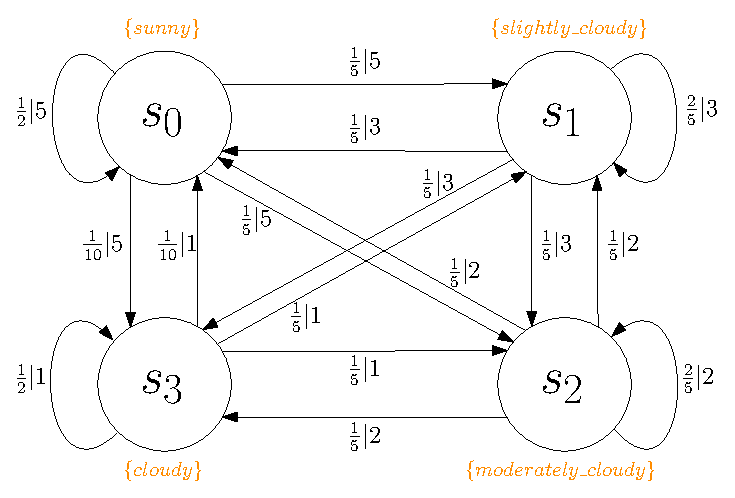
\includegraphics[width=0.6\linewidth]{resources/weather-solar-pannel}
    \caption{MC modeling a daily production of energy (in $kJ$) of solar panels according to weather}
    \label{MCexample}
  \end{figure}
  The way $w$ is defined for this MC yields that when a day is sunny, the installation produces $5 kJ$ during this day, $3 kJ$ when a day is slightly cloudy, $2 kJ$ when a day is moderately cloudy and finally $1 kJ$ when the day is cloudy.
\end{example}

\subsection{Probability of paths of MCs}

\begin{definition}[\textbf{Paths of a MC}] Let $\mathcal{M} = (S, \Delta, w, AP, L)$ be a MC.
A \textit{path} $\pi = s_0 s_1 s_2 \dots$ of $\mathcal{M}$ is a (infinite) sequence of states of the MC such that for all $i \in \mathbb{N}$, $\Delta(s_i, s_{i+1})> 0$. We denote by $Paths(s)$ the set of paths $\pi = s_0s_1s_2\dots$ of $\mathcal{M}$ starting from the state $s \in S$, i.e., such that $s_0 = s$.
\end{definition}
\begin{definition}[\textbf{Finite paths of a MC}]
Let $\mathcal{M} = (S, \Delta, w, AP, L)$ be a MC.
A \textbf{finite} path $\hat{\pi} = s_0 \dots s_n$ of $\mathcal{M}$, with $n \in \mathbb{N}$, is a finite sequence of states of $\mathcal{M}$ such that $\Delta(s_i, s_{i+1}) > 0$ for all $i \in \{0, \dots, n-1\}$.
We denote by $Paths_{fin}(s)$ the set of finite paths $\hat{\pi} = s_0 \dots s_n$ starting from the state $s \in S$, i.e., such that $s_0 = s$
\end{definition}
\begin{definition}[\textbf{Prefixes of paths}]
Let $\mathcal{M} = (S, \Delta, w, AP, L)$ be a MC and $\pi = s_0s_1s_2 \dots$ be a path of $\mathcal{M}$. A prefix of $\pi$ is a finite path $\hat{\pi} = s'_0 \dots s'_n$, with $n \in \mathbb{N}$, such that $s'_i = s_i$ for all $i \in \{0, \dots, n\}$.
The set of all prefixes of $\pi$ is denoted by $pref(\pi)$.
\end{definition}

We are now interested of measuring the probability of events of MCs. These events can be formulated with the notion of \textit{cylinder set}.

\begin{definition}[\textbf{Cylinder set}]
Let $\mathcal{M} = (S, \Delta, w, AP, L)$ be a MC, $s \in S$ be a state of $\mathcal{M}$ and $\hat{\pi} \in Paths_{fin}(s)$ be a finite path of $\mathcal{M}$.
\[Cyl(\hat{\pi})=\{\pi\in Paths(s)\;|\;\hat{\pi}\in pref(\pi) \} \]
\end{definition}

We can express all events with this formulation. For example, the event that consists of a singleton containing just a single path $\pi = s_0s_1\dots$ is given by $\bigcap_{\hat{\pi} \in pref(\pi)} Cyl(\hat{\pi})$

\begin{theorem}\label{theo1}
  Let $\mathcal{M}=(S, \Delta, w, AP, L)$ be a MC and $s \in S$ be a state of $\mathcal{M}$. There exists a unique probability measure $\mathbb{P}_s$ on the
  $\sigma$-algebra over $Paths(s)$ where the probabilities of cylinder sets (i.e., of events) are given by
  \[
    \mathbb{P}_s(Cyl(s_0 \dots s_n)) = \prod_{i = 0}^{n - 1} \Delta(s_i, s_{i+1})
  \]
  where $s_0 = s$ and $n \in \mathbb{N}$.
\end{theorem}
\begin{corollary}
Any event defined using complementation or countable union of cylinder sets are also measurable.
\end{corollary}

\begin{example}[\textit{Probability of paths in a MC modeling a solar panel system}]
  Let $\mathcal{M}_{sp} = (S, \Delta, w, AP, L)$ be the MC of the example \ref{solar-panel}. The probability of sunny weather four days in a row starting on a sunny day is given
  by $\mathbb{P}_{s_0}(Cyl(s_0s_0s_0s_0)) = (\frac{1}{2})^3 = \frac{1}{8}$
\end{example}

\subsection{Objectives in Markov chains}

With this background, we can now introduce some classical problems that consist
of completing an objective in a MC. The first one that we will tackle is the reachability problem.
%\subsubsection{Reachability problem}
\begin{definition}[\textbf{Reachability event}]
  Let $\mathcal{M} = (S, \Delta, w, AP, L)$ be a MC and $T \subseteq S$ be a set of target states. The event of reaching $T$, denoted by $\Diamond T$,
  is defined as a finite union of cylinder sets. Indeed, let $s \in S$ be a state of $\mathcal{M}$ and $Paths_{fin}^T(s)$ be the set of finite paths $\hat{\pi} = s_0 \dots s_n \in Paths_{fin}(s)$, such that for all $i \in \{0, \dots, n-1 \}, \, s_i \not \in T$ and $s_n \in T$,
  \[ \Diamond T = \bigcup_{s_0 \dots s_n \in Paths_{fin}^T(s)} Cyl(s_0 \dots s_n) \]
  As all cylinders of the set $Paths_{fin}^T(s)$ are disjoint (their prefixes are different), we can measure the probability of $\Diamond T$ with:
  \[
    \mathbb{P}_s(\Diamond T) = \sum_{s_0 \dots s_n \in Paths_{fin}^T(s)}  \mathbb{P}_s(Cyl(s_0 \dots s_n))
  \]
\end{definition}
It remains to compute this probability.

\begin{theorem}
Computing $\mathbb{P}_s(\Diamond T)$ for all $s \in S$ can be done in polynomial
time through a linear equations system (cf. appendix \ref{app-reach} for more details).
\end{theorem}

% \begin{example}[\textit{Reachability property in a MC modeling a solar panel system}]
%   Let $\mathcal{M}_{sp}$ be the MC modeling the system of the example \ref{solar-panel}.
%    The probability that a cloudy day eventually comes, starting on a sunndy day, is one, i.e., $\mathbb{P}_{s_0}(\Diamond \{s_3\}) = 1$. Indeed, the underlying graph of $\mathcal{M}_{sp}$ is strongly connected, so reaching any state starting from any state has always a probability $1$.
% \end{example}

Now, we will consider the \textit{cost of paths} of a MC. Furthermore, we
are interrested by the cost of paths to reach $T$. To compute this cost, we use the \textit{truncated sum function}.

\begin{definition}[\textbf{Truncated sum}]
  Let $\mathcal{M}=(S, \Delta, w, AP, L)$ be a MC, $s \in S$ be a state of $\mathcal{M}$, $\pi = s_0s_1s_2\dots \in Paths(s)$ be a path of $\mathcal{M}$ and $T \subseteq S$ be a set of target states.
  The trunacted sum of $\pi$ is the cost to reach $T$ through $\pi$
  for the first time. More formally, the function $TS^T: Paths(s) \rightarrow \mathbb{N} \cup \{\infty\}$ is defined as follows:
	\[
		TS^T(\pi) =
		\begin{cases}
			\sum_{i = 0}^{n-1} w(s_i, s_{i+1}) & \quad \text{if } \forall i \in \{0, \dots, n - 1\}, s_i \not\in T \text{ and } s_n \in T \\
			\infty & \quad \text{else, if } \forall i \in \mathbb{N}, \, s_i \notin T
		\end{cases}
	\]
\end{definition}
With this function, it is now possible to introduce the concept of the
expected cost of paths of a MC to reach a set of targets as well as
the probability of reaching this target set with a cost bounded.

\begin{definition}[\textbf{Expected cost of paths of a MC for reachablity properties}]
	Let $\mathcal{M} = (S, \Delta, w, AP, L)$ be a MC, $s \in S$ be a state of $\mathcal{M}$ and $T \subseteq S$ be a set of target states. We define the expected cost to reach $T$, i.e., $\mathbb{E}_s(\Diamond T)$, corresponding to \textit{the expected truncated sum of paths from $s$ to reach $T$} as follows:
	\begin{itemize}
	\renewcommand{\labelitemi}{\tiny$\bullet$}
	\item If $\mathbb{P}_s(\Diamond T) < 1$, then $\mathbb{E}_s(\Diamond T) = \infty$.%(par la propriété \ref{prop-ts}).
	\item Else, if $\mathbb{P}_s(\Diamond T) = 1$, then:
	\[
    \mathbb{E}_s(\Diamond T) = \sum_{c = 0}^\infty c \cdot \mathbb{P}_s(\{\pi \in Paths(s) \; | \; TS^T(\pi) = c \})
  \]
	\end{itemize}
\end{definition}

An equivalent characterisation of the expected cost from $s \in S$ to $T$ in case of $\mathbb{P}_s(\Diamond T) = 1$ is given by
\[
  \mathbb{E}_s(\Diamond T) = \sum_{\hat{\pi} \in Paths_{fin}^T(s)} \mathbb{P}_s(Cyl(\hat{\pi})) \cdot TS^T(\hat{\pi})
\]
with $Paths^T_{fin}(s)$, the set of finite paths $\hat{\pi} = s_0 \dots s_n \in Paths_{fin}(s)$  such that for all $i \in \{0, \dots, n-1\}, s_i \not \in T$ and $s_n \in T$. As we can measure the probability of cylinder sets of finite paths of $\hat{\pi} \in Paths_{fin}^T(s)$, we can compute $\mathbb{E}_s(\Diamond T)$.

\begin{theorem}
  Computing $\mathbb{E}_s(\Diamond T)$ for all $s \in S$ can be done in polynomial time through a linear equations system (cf. appendix \ref{app-expMC} for more details).
\end{theorem}

The last concept that we will define in MCs is the cost bounded reachability.

\begin{definition}[\textbf{Cost bounded reachability probability}]
	Let $\mathcal{M} = (S, \Delta, w, AP, L)$ be a MC, $s \in S$ be a state of $\mathcal{M}$, $T \subseteq S$ be a set of target states and $l \in \mathbb{N}$, a length threshold.
  The \textit{probability to reach $T$ from $s$ with a cost bounded} by the threshold $l$ is defined as follows:
	\[
    \mathbb{P}_s(\Diamond_{\leq l} T) = \mathbb{P}_s(\{\pi \in Paths(s) \; | \; TS^T(\pi) \leq l \})
  \]
\end{definition}
The event $\{\pi \in Paths(s) \; | \; TS^T(\pi) \leq l \}$ is actually measurable
in the unfolded MC until $l$.
\begin{theorem}
  The probability of the cost bounded reachability to a set of target states $T \subseteq S$ from a state $s \in S$ can be computed in pseudo-polynomial time in the size of $\mathcal{M}$ and $l$, through an unfolding of $\mathcal{M}$ until $l$.
\end{theorem}

Intuitively, we unfold $\mathcal{M}$ by recording in each state the cost of
current paths. The new set of target states in the unfolded MC is the set of
target states in $\mathcal{M}$ that have a current cost less than $l$ (cf.
appendix \ref{app-cbrMC} for more details). Finally, it remains to compute the probability to
reach these new target states in the unfolded MC. \\

Now, we can define what is a Markov decision process and introduce the concept of strategy that is the pillar concept of resolving objective problems in such models.

\section{Markov decision processes}
Markov decision processes are systems that modelise situations describing both non-deterministic and stochastic evolution. Indeed, in comparison with Markov chains, Markov decision processes require a decision making to go from a state of the model to its successors. After that, the system evolve following the probability distribution formed by this state and the decision taken.

\begin{definition}[\textbf{Markov decision process}]
	A \textit{Markov decision process}, (denoted by \textbf{MDP}) is defined by a tuple $\mathcal{M}  = (S, A, \Delta, w, AP, L)$ where
	\begin{itemize}
		\item $S$ is a countable set of states,
		\item $A$ is a countable set of actions ; we denote by $A(s) \in 2^A$  the set of enabled actions when the system is in state $s$ and for all $s \in S$,
    we have $A(s) \neq \emptyset$,
		\item $\Delta: S \times A \times S \rightarrow [0, 1] \cap \mathbb{Q}$ is the probability transition function such that
		\begin{flalign*}
			&\forall s \in S, \; \forall \alpha \in A(s), \; \sum_{s' \in S} \Delta(s, \alpha, s') = 1 \\
			\text{and } &\forall s, s' \in S, \; \forall \alpha \in A \setminus A(s), \; \Delta(s, \alpha, s') = 0
		\end{flalign*}

			where $\Delta(s, \alpha, s')$ defines the probability of going from $s$ to $s'$ in one transition when the action $\alpha \in A(s)$ is chosen,
    \item $w: A \rightarrow \mathbb{N}_0$ %est la fonction
        %de poids associant à chaque transition un coût strictement positif.
      is a weight function that links a strictly positive cost to each action,
    \item $AP$ is a set of atomic propositions, and
    \item $L: S \rightarrow 2^{AP}$ is a labeling function.
	\end{itemize}
  \textit{Remark: }again, $AP$ and $L$ can be ommited. In that case, we consider that $AP=S$ and $L$ is the natural labeling of each state, i.e., for all state $s \in S$, $L(s) = \{s\}$.
\end{definition}

\begin{property}
  Let $\mathcal{M} = (S,A, \Delta, w, AP, L)$ be a MDP, $s \in S$ be a state of $\mathcal{M}$ and $\alpha \in A(s)$ be an enabled action of the state $s$. The transition function $\Delta$ defines a probability distribution $\Delta_{s, \alpha}: S \rightarrow \mathcal{D}(S), \, s' \mapsto \Delta(s, \alpha, s')$ on $S$.
\end{property}
\begin{property}
  A MC is essentially a MDP where, for each state $s$, $|A(s)| = 1$.
\end{property}

We will now introduce some useful notations.

\begin{notation}
  Let $\mathcal{M}=(S, A, \Delta, w, AP, L)$ be a MDP,
  \begin{itemize}
    \item $Pred(s) = \{ s' \in S \; | \; \exists \alpha \in A(s'), \, \Delta(s', \alpha, s) > 0 \}$ is the set of predecessors of the state $s \in S$ in the the MDP,
    \item $Succ(s) = \{ s' \in S \; | \; \exists \alpha \in A(s), \, \Delta(s, \alpha, s') > 0 \}$ is the set of successors of the state $s \in S$ in the MDP and
    \item $Succ(s, \alpha) = \{ s' \in S \; | \; \Delta(s, \alpha, s') > 0 \}$
      is the set of $\alpha$-successors of the state $s \in S$ in the MDP, i.e., the set of possible successors of $s$ when the action $\alpha$ is chosen
  \end{itemize}
\end{notation}

%The underlying graph of a MDP $\mathcal{M}$ is a directed graph where vertices are states of $\mathcal{M}$ and each edge starting from a state $s$ to one of its successor $s'$ exists if and only if there exists an enabled action $\alpha$
%of $s$ such that $\Delta(s, \alpha, s') > 0$. For the other elements of the tuple defining $\mathcal{M}$, the graph is essentially caracterised the same way as for a MC.
We can represent a MDP with its underlying directed graph, the same way as for a MC, with the exception that each vertex representing a state $s$ has outgoing edges to intermediate vertices representing enabled actions of $s$ and, for each enabled action $\alpha$ of $s$, edges go from the vertex representing $\alpha$ to the vertices representing $\alpha$-successors of $s$.

\begin{notation}[\textit{Size of a MDP}]
  A MDP $\mathcal{M}=(S, A, \Delta, w, AP, L)$ is called \textit{finite} if its states space $S$ is finite. The size of $\mathcal{M}$ corresponds to the size
  of the set $\{(s, \alpha, s') \in S \times A \times S \; | \; \Delta(s, \alpha, s') > 0 \}$, i.e., the number of outgoing edges of vertices representing actions in the underlying graph of $\mathcal{M}$.
\end{notation}

\begin{example}\label{simple-mdp}
  Let $\mathcal{M} = (S, A, \Delta, w, AP, L)$ be the MDP of the figure \ref{mdp01}. We have that $S = \{s_0, s_1, s_2\}$, $A = \{\alpha, \beta, \gamma\}$ and $AP=\{a, b\}$. If the system currently is in state $s_0$, labeled with $L(s_0) = \{a\}$, the only action available is $\beta$ (because $A(s_0) = \{\beta\}$).
  The cost of choosing $\beta$ is $w(\beta) = 3$.
  So, the system evolves following the probability distribution defined by $\Delta_{s_0, \beta}$: it has a probability of $\frac{1}{2}$
  to go to its $\beta$-successor $s_1$ and a same probability to go to its $\beta$-successor $s_2$. Let assume that the system evolves to the state $s_2$, a state with no label ($L(s_2) = \emptyset$). So, in that case, the system has two possible decisions: $\alpha$ or $\gamma$ (because $A(s_2) = \{\alpha, \gamma\}$). If $\alpha$ is chosen, the system returns to $s_2$ with a probability one and a cost of $w(\alpha) = 5$. Else, if $\gamma$ is chosen, the system goes to $s_0$ with a probability one and a cost of $w(\gamma) = 2$.
  \begin{figure}[h!]
    \centering
    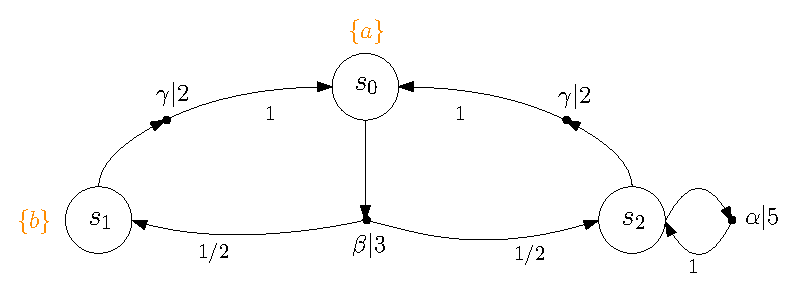
\includegraphics[width=0.7\linewidth]{resources/simple-mdp}
    \caption{MDP with $3$ states, $3$ actions and $2$ atomic propositions}\label{mdp01}
  \end{figure}
\end{example}

\subsection{Strategies in MDPs}
In order to resolve nondeterminism inside MDPs, we need the notions of paths in MDPs and strategies.
\begin{definition}[\textbf{Paths in a MDP}]
  Let $\mathcal{M}=(S, A, \Delta, w, AP, L)$ be a MDP and the transition relation
  \[\rightarrow \; =  \{ (s, \alpha, s') \in S \times A \times S \; | \; \Delta(s, \alpha, s') > 0 \}, \,\]
	a path $\pi$ of $\mathcal{M}$ is defined as a sequence of states
	\[ \pi = s_0 \xrightarrow{\alpha_1} s_1 \xrightarrow{\alpha_2} s_2 \xrightarrow{\alpha_3} \dots \]
	Let $s \in S$ be a state of $\mathcal{M}$, we denote by $Paths(s)$ the set of
	paths of $\mathcal{M}$ starting from the state $s$, i.e., such that $s_0 = s$.
\end{definition}
In opposition of MCs, there is no probabilistic space defined on paths of MDPs.
This is related to nondeterminism linked to the choices of actions possible when the system is in a state. We need strategies to resolve nondeterminism.
\begin{definition}[\textbf{Histories}]
	Let $\mathcal{M} = (S, A, \Delta, w, AP, L)$ be a MDP. A \textit{history} of $\mathcal{M}$
	is a finite sequence of states $(s_0 \dots s_n) \in S^+$ where for all
	$i \in \{1, \dots, n \}, \; \exists \alpha \in A(s_{i-1})$ such that $\Delta(s_{i-1}, \alpha, s_i) > 0$.
	A history is the sequence of state that brought the state $s_0$ to the state $s_n$ along a path of $\mathcal{M}$. The set of histories of $\mathcal{M}$  is given by $\mathcal{H}(S)$.
\end{definition}

These notions allow to introduce strategies in MDPs.

\begin{definition}[\textbf{Pure strategy}]
Let $\mathcal{M} = (S, A, \Delta, w, AP, L)$ be a MDP. A \textit{strategy} (also named \textit{policy} or \textit{scheduler} in literature) for $\mathcal{M}$
	is a function
	$\sigma: \mathcal{H}(S) \rightarrow A$
	that selects, for a given history $h = (s_0 \dots s_n) \in \mathcal{H}(S)$, an enabled action of $s_n$, i.e., $\sigma(s_0 \dots s_n) = \alpha \in A(s_n)$.
	The path $\pi = s_0 \xrightarrow{\alpha_1} s_1 \xrightarrow{\alpha_2} s_2 \xrightarrow{\alpha_3} \dots$
	is a $\sigma$-path iff $\alpha_i = \sigma(s_0 \dots s_{i-1})$
	for all $i \in \mathbb{N}_0$. The set of $\sigma$-paths starting from the state $s \in S$ is given by $Paths^\sigma(s)$.
\end{definition}
The strategies that we study here are \textit{pure}, i.e., each action is chosen by strategy with probability one. We will see later that \textit{randomised} strategies exist and are essential to resolve some type of problems in MDP. \\

If a strategy controls the decisions of a MDP, then the nondeterminism is solved
and the MDP acts like a MC. Actually, a MDP $\mathcal{M}$ controlled by a strategy $\sigma$ can be formalised as a MC $\mathcal{M}^\sigma$.

\begin{definition}[\textbf{Markov chain induced by strategy}]
Let $\mathcal{M} = (S, A, \Delta, w, AP, L)$ be a MDP and $\sigma$ be a strategy for
$\mathcal{M}$. The MC induced by $\sigma$ is given by
$ \mathcal{M}^\sigma = (\mathcal{H}(S), \Delta^\sigma, w^\sigma, AP, L^\sigma) $, where, for all history
$h = s_0 s_1 \dots s_n$ of $\mathcal{M}$,
\begin{itemize}
\item $\Delta^\sigma(h, h . s_{n+1}) = \Delta(s_n, \sigma(h), s_{n+1})$
\item $w^\sigma(h, h . s_{n+1}) = w(\sigma(h))$
\item $L^\sigma(h . s_{n+1}) = L(s_{n+1})$
\end{itemize}
\end{definition}

\begin{property}
  Let $\mathcal{M}$ be a MDP, $\sigma$ be a strategy on $\mathcal{M}$ and $s\in S$ be a state of $\mathcal{M}$. There exists a bijection between the
  set $Paths^\sigma(s)$ on $\mathcal{M}$ and the set $Paths(s)$ on $\mathcal{M}^\sigma$
\end{property}

As the propability of events in a MC is measurable, the probability of events in a MDP controlled by strategy is also measurable.
\begin{notation}
  We denote by $\mathbb{P}_s^\sigma$ the probability measure defined on paths starting from the state $s$ of the Markov chain induced by the strategy $\sigma$.
\end{notation}

Markov chains induced by such (infinite memory) strategies can be seen as forests of trees representing an infinite unfolding of the MDP where actions are controlled by strategy (this is due to the fact that the set of histories of a MDP is infinite). So, such induced MCs have infinite size. Actually, such strategies are not easy to use in practice because it requires to
know the complete history of the system to decide which action to choose. \textit{Finite memory strategies} allow to avoid this problem.

\begin{definition}[\textbf{Finite memory strategy}]
Let $\mathcal{M} = (S, A, \Delta, AP, L)$ be a MDP.
A \textit{finite memory strategy} $\sigma = (Q, \sigma_\alpha, \delta, \delta_0)$ is a \textit{Moore machine} where
\begin{itemize}
	\item $Q$ is a finite set of \textit{modes},
	\item $\sigma_\alpha: Q \times S \rightarrow A$ is a function that that choose, for any $s \in S$, an action $\alpha \in A(s)$ following a mode $q \in Q$ in which the machine currently is,
	\item $\delta: Q \times S \rightarrow Q$ is the transition function,
	\item $\delta_0: S \rightarrow Q$ is the function that chooses the initial mode of the machine following a state $s \in S$ of the MDP from which the machine is initialised.
\end{itemize}
\end{definition}

\begin{definition}[\textbf{Product of a MDP by a strategy}]
Let $\mathcal{M} = (S, A, \Delta, w, AP, L)$ be a MDP and $\sigma = (Q, \sigma_\alpha, \delta, \delta_0)$ be a finite memory strategy for $\mathcal{M}$.
The product of $\mathcal{M}$ by $\sigma$ is given by
\[ \mathcal{M} \times \sigma = \mathcal{M}^\sigma = (S \times Q, \Delta^\sigma, w^\sigma, AP, L^\sigma) \]
where $\mathcal{M}^\sigma$ is the MC induced by the finite memory strategy $\sigma$ and where,
for all states $s, s' \in S$ and for all modes $q, q' \in Q$ of the strategy,
\begin{itemize}
	\item $\Delta^\sigma((s, q), (s', q')) =
	\begin{cases}
	\Delta(s, \sigma_\alpha(q, s), s') & \text{if } \delta(q, s) = q'\\
	0  & \text{else}
	\end{cases}$
  \item $w^\sigma((s, q), (s', q')) = w(\sigma_\alpha(q, s))$
  \item $L^\sigma(s, q) = L(s)$
\end{itemize}
\end{definition}

\begin{example}[\textit{Product of a MDP by a strategy}]
  Let $\mathcal{M}=(S, A, \Delta, w, AP, L)$ be the MDP of the example \ref{simple-mdp} and $\sigma = (Q, \sigma_\alpha, \delta, \delta_0)$ be the
  finite memory strategy of the figure \ref{finite_mem_strat}.
  \begin{figure}[h!]
    \centering
    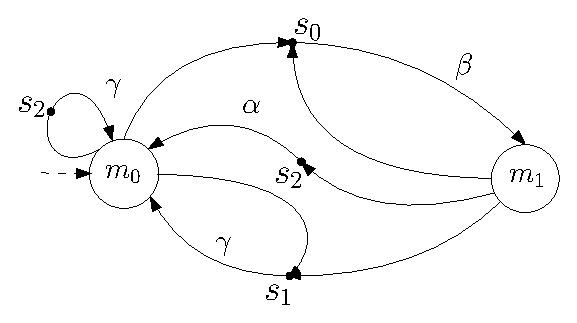
\includegraphics[width=0.4\linewidth]{resources/strategy}
    \caption{Finite memory strategy for $\mathcal{M}$ with $2$ modes}\label{finite_mem_strat}
  \end{figure}

  We assume that for all $s \in S$, $\delta_0(s) = m_0$. The strategy simply consists in choosing once $\alpha$ when the system enters in the state $s_2$ and choosing $\gamma$ just after that, to return to $s_0$. The MC induced by the product of $\mathcal{M}$ by $\sigma$ is given in the figure
  \ref{inducedMC}.
  \begin{figure}[H]
    \centering
    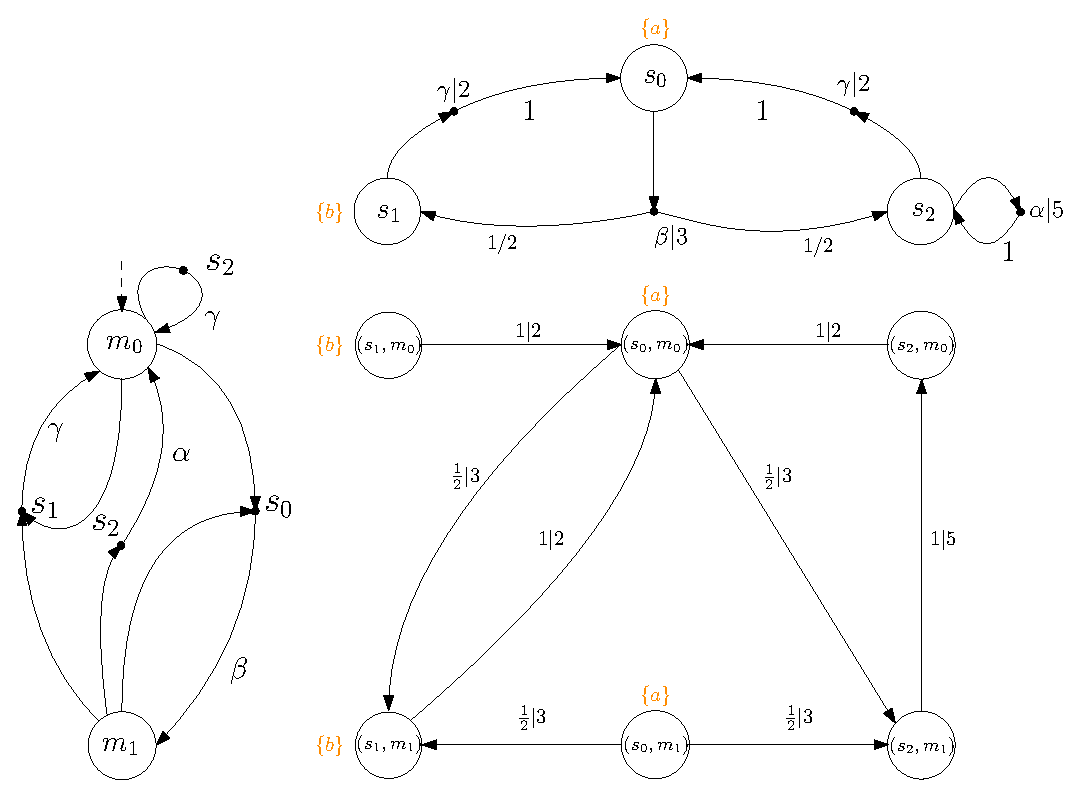
\includegraphics[width=0.55\linewidth]{resources/inductedmarkov}
    \caption{Product of $\mathcal{M}$ by $\sigma$}\label{inducedMC}
  \end{figure}
\end{example}

Finally, the last type of strategy that we will see is a particular case of finite memory strategies, where strategies have only one mode.
In that case, the action chosen by a such strategy only depends on the current state of the system.

\begin{definition}[\textbf{Memoryless strategy}]
  Let $\mathcal{M}=(S, A, \Delta, w, AP, L)$ be a MDP. A \textit{memoryless strategy} is a function
  $
    \sigma: S \rightarrow A
  $ that links each state $s$ of $\mathcal{M}$ to an enabled action $\alpha \in A(s)$ of this state.
\end{definition}

\begin{property}
  A memoryless strategy is a finite memory strategy with only one mode.
\end{property}

\subsection{Objectives in Markov decision processes}
The resolution of problems in MDPs will be done through strategies that will choose the optimal actions to complete different objectives. As for the MC, we will first address the \textit{stochastic reachability problem} in a MDP.
\begin{definition}[\textbf{SR problem}]
  Let $\mathcal{M}=(S, A, \Delta, w, AP, L)$ be a MDP, $s \in S$ be a state of $\mathcal{M}$, $T$ be a set of target states and $\alpha \in [0, 1]$ be
  a probability threshold. The \textit{stochastic reachability} (SR) problem consists
  of deciding if a strategy $\sigma$ exists such that
  \[
    \mathbb{P}_s^\sigma(\Diamond T) \geq \alpha
  \]
\end{definition}

\begin{theorem}
  The SR-problem can be decided in polynomial time in the size of $\mathcal{M}$
  through a linear program, by building a pure memoryless strategy that gives the optimal actions to reach $T$ from every state $s \in S$ (cf. appendix \ref{app-sr} for more details).
\end{theorem}

Before introducing the following, we will first introduce the \textit{truncated sum} of paths of MDPs in order to compute the cost of paths of a MDP.

\begin{definition}[\textbf{Truncated sum for MDPs}]
	Let $\mathcal{M} = (S, A, \Delta, w, AP, L)$ be a MDP, $s \in S$ be a state of $\mathcal{M}$, $T \subseteq S$ be a set of target states and
	$\pi = s_0 \xrightarrow{\alpha_1} s_1 \xrightarrow{\alpha_2} s_2 \xrightarrow{\alpha_3} \dots \in Paths(s)$ be a path of
	$\mathcal{M}$ starting from $s$. The truncated sum $TS^T: Paths(s)
	\rightarrow \mathbb{N} \cup {\infty}$ of the path $\pi$ is defined as follows:
	\[
		TS^T(\pi) =
		\begin{cases}
			\sum_{i = 1}^{n} w(\alpha_i) & \quad \text{if } \forall i \in \{0, \dots, n - 1\}, s_i \notin T \text{ and } s_n \in T \\
			\infty & \quad \text{else, if $ \forall i \in \mathbb{N}, \, s_i \not\in T$}
		\end{cases}
	\]

\end{definition}

By considering the cost of paths of a MDP, we are now interested by building some
strategies inducing the shortest path to go from one state to a set of target
states. The notion of shortest path in a MDP is not as obvious as in a graph due to the uncertainty linked to the stochastic environment.
The stochastic shortest path problem in a MDP can be approached in different
ways. We will first approach the \textit{stochastic shortest path expectation} problem and
then approach the \textit{stochastic shortest path percentile} problem. \\

Since the probability of paths induced by strategy is measurable and
since the cost of theses paths is computable via the trunacted sum function, we can
compute the expected length of paths that reach a set of target states using a strategy and more particulary build the strategy that will minimise the expected length of these paths.

\begin{definition}[\textbf{SSP-E problem}]
Let $\mathcal{M}=(S, A, \Delta, w, AP, L)$ be a MDP, $s \in S$ be a state of $\mathcal{M}$,
$T \subseteq S$ be a set of target states and $l \in \mathbb{N}$ be a paths length
threshold of paths. The \textit{stochastic shortest path expectation} (SSP-E) problem
consists of deciding if a strategy $\sigma$ exists such that
\[
  \mathbb{E}^\sigma_s(\Diamond T) \leq l
\]
% i.e., if there exists a strategy $\sigma$ such that the expected length of paths starting in the state $s$ in the MC induced by this strategy is lower than the length threshold $l$.
where $\mathbb{E}_s^\sigma(\Diamond T)$ corresponds to the expected cost of paths starting from $s$ in the MC induced by $\sigma$.
\end{definition}

\begin{theorem}
  The SSP-E problem can be decided in polynomial time in the size of $\mathcal{M}$, through a linear program by building a pure memoryless strategy that gives the optimal actions to minimise the expected cost of paths to reach $T$ from every state $s \in S$ (cf. appendix \ref{app-sspe} for more details).
\end{theorem}

Finally, the last problem that we will present in this chapter is the
\textit{stochastic shortest path percentile} problem. For this problem, we will
be interested to decide if there exists a strategy that allow to reach a set of target states with
a cost bounded by a high probability threshold.

\begin{definition}[\textbf{SSP-P problem}]
  Let $\mathcal{M} = (S, A, \Delta, w, AP, L)$ be a MDP, $s \in S$ be a state of
  $\mathcal{M}$, $T \subseteq S$ be a set of target states, $l \in \mathbb{N}$
  be a paths length threshold and $\alpha \in [0, 1]$ be a probability
  threshold. The \textit{stochastic shortest path percentile} (SSP-P) problem
  consists of deciding if there exists a strategy $\sigma$ such that
  \[
    \mathbb{P}_s^\sigma (\Diamond_{\leq l} T) \geq \alpha
  \]
\end{definition}

\begin{theorem}
  The SSP-P problem can be decided in pseudo-polynomial time in the size of $\mathcal{M}$ and $l$ by building a pure finite memory strategy. This strategy is built by unfolding the MDP $\mathcal{M}$ from the state $s$ until $l$ and by resolving the SR problem on this unfolded MDP.
\end{theorem}

\begin{definition}[\textbf{Unfolded MDP until a bounded length}] Let
  $\mathcal{M} = (S, A, \Delta, w, AP, L)$ be a MDP, $s^* \in S$ be a state of
  $\mathcal{M}$, $T \subseteq S$ be a set of target states of $\mathcal{M}$ and $l \in \mathbb{N}$ be a paths length threshold.
  Unfolding $\mathcal{M}$ from $s^*$ until $l$ can be done as follows: \\
  We build $\mathcal{M}_l = (S_l, A_l, \Delta_l, w, AP, L_l)$ for the subset $T_l \subseteq S_l$ where
  \begin{itemize}
  \item $S_l$ is composed of states $(s, v)$ where $s \in S$ et $v \in \{0, \dots, l\} \cup \{\bot\}$.
  We consider that $\bot > l$, with $\bot + v = \bot$ for all $v \in \{0, \dots, l\}$.
  Intuitively, $v$ records the cost of paths while unfolding $\mathcal{M}$.
  As we unfold $\mathcal{M}$ from $s^*$, we have that
  $(s, 0) \not \in S_l$ for all $s \in S$ such that $s \neq s^*$.
  \item For each $\alpha \in A$, we have that $\alpha \in A_l$ and for all $(s, v) \in S_l$, $A_l(s, v) = A(s)$.
  \item $\Delta_l: S_l \times S_l \rightarrow [0, 1]$ is the probability transition function given by:\\
  $\text{Forall } (s, v), (s', v') \in S_l \text{ and for all } \alpha \in A(s),$
  \[
  \Delta_l((s, v), \alpha, (s', v')) =
  \begin{cases}
  	\Delta(s, \alpha, s') & \quad \quad \text{ if } v' = v + w(\alpha) \leq l \text{ or}\\
  	 & \quad \quad \text{ if } v' = \perp \text{ and } v+w(\alpha) > l \\
  	0 & \quad \quad \text{ else}
  \end{cases}
  \]
  \item $L_l:S_l \times \mathbb{N} \rightarrow AP \mapsto L_l(s, v) = L(s)$.
  \item Target states are states of
  $T_l = \{(s, v) \;|\; s \in T \wedge v \leq l \}$.
  \end{itemize}
  \textit{Remark}: since all state $(s, v) \in S_l$ such that $v = \bot$ can never reach $T_l$, it is not useful to keep these states in the unfolded MDP $\mathcal{M}_l$. So, we can replace all these states in $S_l$ with a unique state $\bot$ such that, for all $(s, v) \in S_l$ such that $v \neq \bot$ and for all $\alpha \in A(s)$ such that $v + w(\alpha) > l$,
  $\Delta_l((s, v), \alpha, \bot) = 1$. Then, we define a new action $\alpha_\bot \in A_l$ with an arbitrary weight that will allow a self-loop for $\bot$, i.e., $\Delta_l(\bot, \alpha_\bot, \bot)=1$.
\end{definition}

\begin{example}[\textit{Unfold a MDP}]
  Let $\mathcal{M} = (S, A, \Delta, w, AP, L)$ be the MDP of the example \ref{simple-mdp}.
  This MDP can be unfolded from the state $s_0$ until the threshold $l = 8$ for the target states set $\{s_1\}$ (cf. figure \ref{unfolding}).
  \begin{figure}[h!]
    \centering
    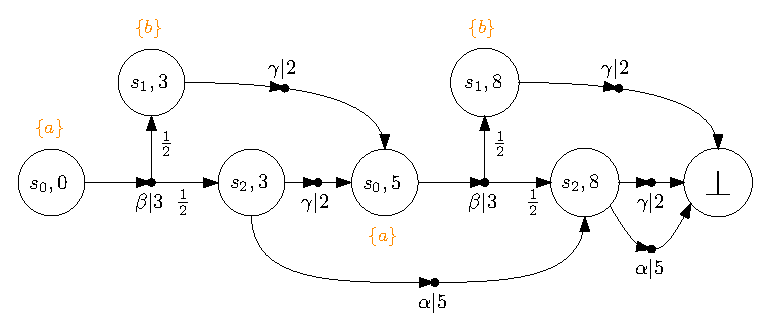
\includegraphics[width=0.8\linewidth]{resources/unfolding}
    \caption{$\mathcal{M}$ unfolded from $s_0$ until $l=8$ for $\{s_1\}$}\label{unfolding}
  \end{figure}
  The highlighted strategy in the figure \ref{unfolding} is the memoryless strategy that resolves the SR problem in $\mathcal{M}_l$. This strategy is the
  same as the one that resolves the SSP-P problem in $\mathcal{M}$ and is thus finite memory in $\mathcal{M}$.
\end{example}
